\documentclass[tikz,border=8pt]{standalone}
% Shared look for every TikZ diagram. Load with \input{../../tools/tikz-style.tex}
\usepackage[sfdefault]{roboto}
\usetikzlibrary{arrows.meta, positioning, shapes.geometric, calc, fit, backgrounds}
\definecolor{cblue}{HTML}{4C78A8}
\definecolor{corange}{HTML}{F58518}
\definecolor{cgreen}{HTML}{54A24B}
\definecolor{cred}{HTML}{E45756}
\definecolor{cpurple}{HTML}{B279A2}
\definecolor{cgrey}{HTML}{6B6B6B}
\tikzset{
  every picture/.style={font=\sffamily, line width=1.2pt},
  box/.style={draw=#1, fill=#1!12, rounded corners=4pt, align=center, inner sep=7pt, minimum height=1.1cm},
  box/.default=cgrey,
  arrow/.style={-{Stealth[length=3mm]}, draw=cgrey, line width=1.4pt},
  title/.style={font=\sffamily\bfseries\Large},
  note/.style={font=\sffamily\small, text=cgrey, align=center},
}
\AtBeginDocument{\hyphenpenalty=10000 \exhyphenpenalty=10000}

% The Nyquist contour of the heading loop: up the imaginary axis, round the right half-plane on a huge half circle,
% clockwise. A tiny half circle steps round the double pole of L(s) at s = 0 on its right, so that pole lies outside.
\begin{document}
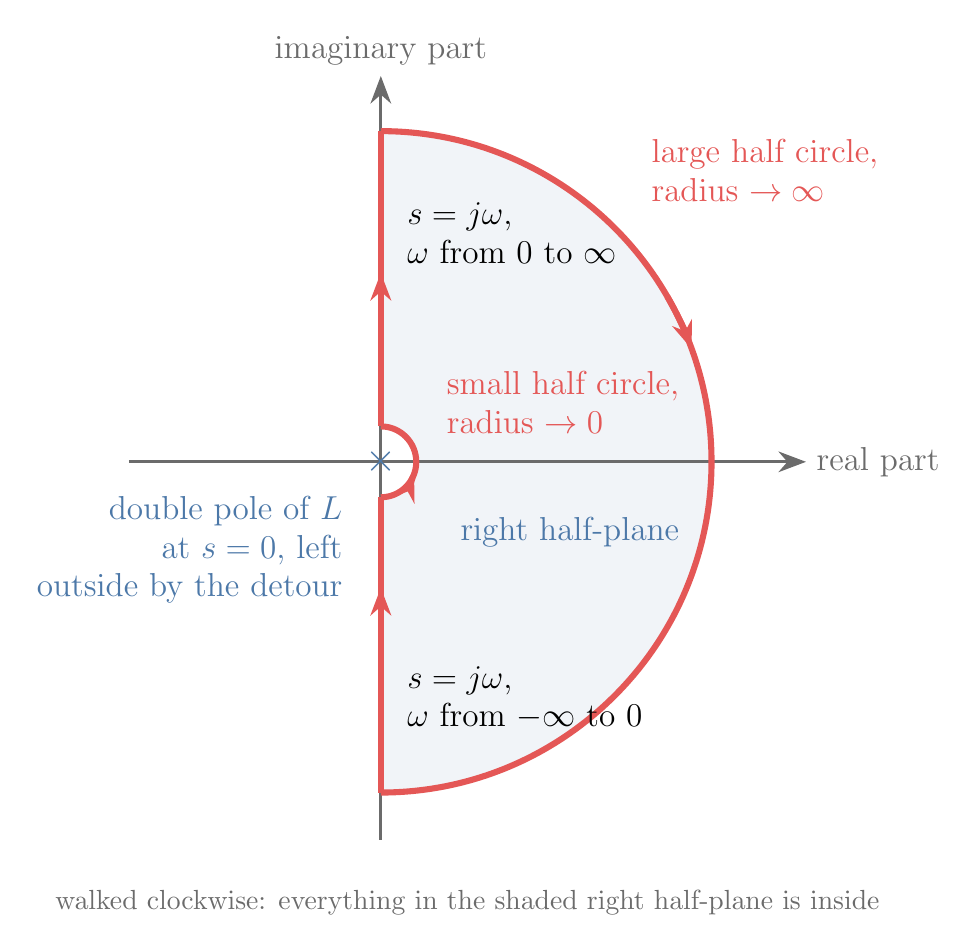
\begin{tikzpicture}[every node/.append style={font=\large}, >={Stealth[length=3.5mm]}]
  \fill[cblue!8] (0,-4.2) -- (0,-0.45) arc (-90:90:0.45) -- (0,4.2) arc (90:-90:4.2) -- cycle;
  \draw[cgrey, line width=1pt, ->] (-3.2,0) -- (5.4,0) node[right] {real part};
  \draw[cgrey, line width=1pt, ->] (0,-4.8) -- (0,4.9) node[above] {imaginary part};
  % the contour
  \draw[cred, line width=2.2pt] (0,0.45) -- (0,4.2);
  \draw[cred, line width=2.2pt] (0,4.2) arc (90:-90:4.2);
  \draw[cred, line width=2.2pt] (0,-4.2) -- (0,-0.45);
  \draw[cred, line width=2.2pt] (0,-0.45) arc (-90:90:0.45);
  \draw[cred, line width=2.2pt, ->] (0,1.6) -- (0,2.4);
  \draw[cred, line width=2.2pt, ->] (0,-2.4) -- (0,-1.6);
  \draw[cred, line width=2.2pt, ->] ({4.2*cos(30)},{4.2*sin(30)}) arc (30:20:4.2);
  \draw[cred, line width=2.2pt, ->] ({0.45*cos(-30)},{0.45*sin(-30)}) arc (-30:-20:0.45);
  % poles of L
  \node[font=\Large, text=cblue] at (0,0) {$\times$};
  \node[text=cblue, anchor=north east, align=right] at (-0.35,-0.3) {double pole of $L$\\at $s = 0$, left\\outside by the detour};
  % labels
  \node[anchor=west, align=left] at (0.2,2.9) {$s = j\omega$,\\$\omega$ from 0 to $\infty$};
  \node[anchor=west, align=left] at (0.2,-3.0) {$s = j\omega$,\\$\omega$ from $-\infty$ to 0};
  \node[anchor=west, align=left, text=cred] at (3.3,3.7) {large half circle,\\radius $\to \infty$};
  \node[anchor=west, align=left, text=cred] at (0.7,0.75) {small half circle,\\radius $\to 0$};
  \node[text=cblue] at (2.4,-0.9) {right half-plane};
  \node[note, font=\normalsize] at (1.1,-5.6) {walked clockwise: everything in the shaded right half-plane is inside};
\end{tikzpicture}
\end{document}
